%auto-ignore
\section{Introduction}
\label{sec:intro}


These instructions are for authors submitting papers to the NAACL-HLT 2021 conference using \LaTeX. They are not self-contained. All authors must follow the general instructions for *ACL proceedings,\footnote{\url{http://acl-org.github.io/ACLPUB/formatting.html}} as well as the newly introduced formatting guidelines for an optional ethics/broader impact section (see the conference website at \url{https://2021.naacl.org/}).  This document contains additional instructions for the \LaTeX{} style files.

The templates include the \LaTeX{} source of this document (\texttt{naacl2021.tex}),
the \LaTeX{} style file used to format it (\texttt{naacl2021.sty}),
an ACL bibliography style (\texttt{acl\_natbib.bst}),
an example bibliography (\texttt{custom.bib}),
and the bibliography for the ACL Anthology (\texttt{anthology.bib}).

\paragraph{Engines}

To produce a PDF file, pdf\LaTeX{} is strongly recommended (over original \LaTeX{} plus dvips+ps2pdf or dvipdf). Xe\LaTeX{} also produces PDF files, and is especially suitable for text in non-Latin scripts. 

\subsection{Equations}

equation \url{https://www.latexlive.com}
\begin{eqnarray}
	a  =  b + c \\
	=  y - z \\
	= \frac{p(x,y)}{p(y)}
\end{eqnarray}

 
\subsection{Graphics}

 \begin{figure}[h!]
	\centering	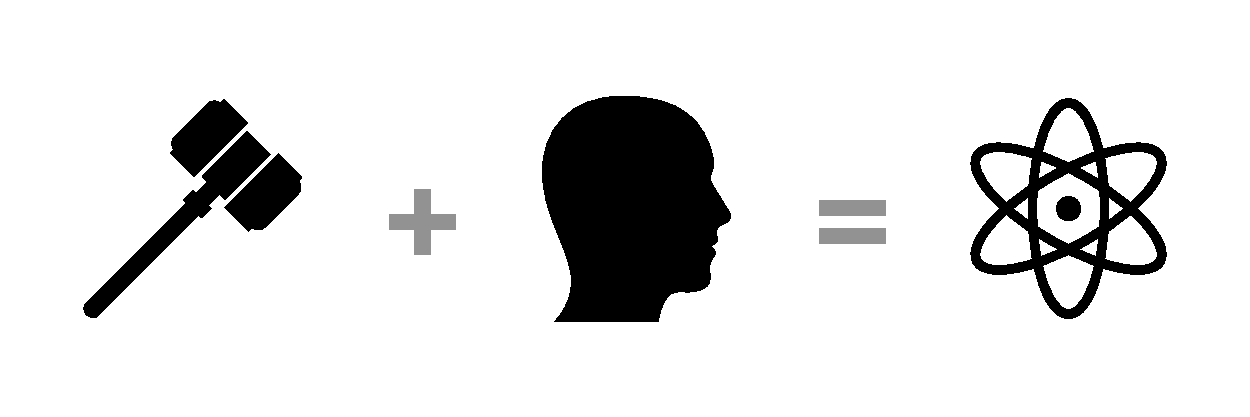
\includegraphics[width=0.5\textwidth]{wisdom.pdf}
	\caption{Physically increasing wisdom.}
	\label{fig:wisdom}
\end{figure}

\begin{figure}[htbp]
	\hspace{-40pt}
	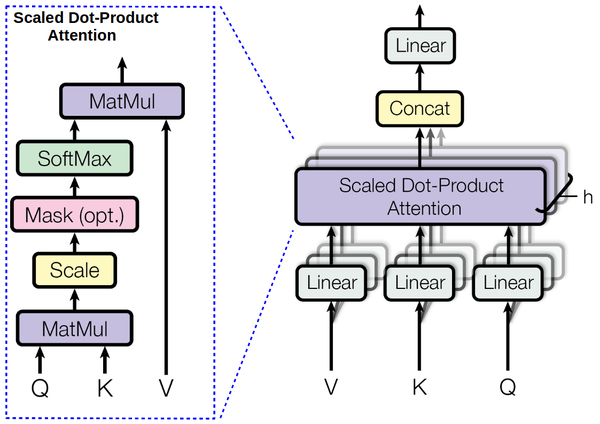
\includegraphics[width=0.6\textwidth]{MultiHead.png}
	\caption{ (左侧表名应为Figure) Multi-Head Attention consists of h attention layers running in parallel.}
	\label{fig:MultiHead}
\end{figure}





